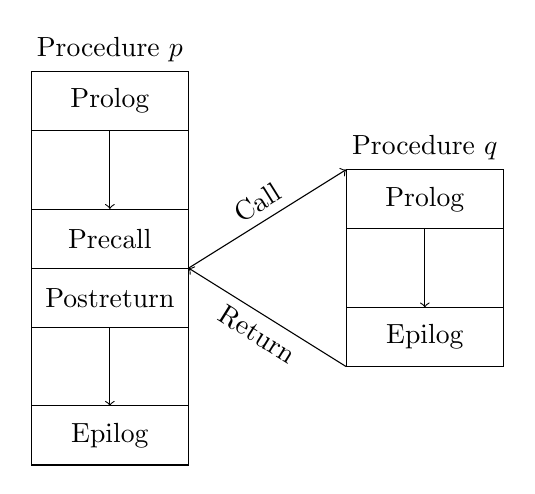
\begin{tikzpicture}
    \draw (0,0) rectangle ++(2, 0.75) node[pos=.5]{Epilog};
    \draw (0,0.75) rectangle ++(2, 1) node[pos=.5]{};
    \draw (0,1.75) rectangle ++(2, 0.75) node[pos=.5]{Postreturn};
    \draw (0,2.5) rectangle ++(2, 0.75) node[pos=.5]{Precall};
    \draw (0,3.25) rectangle ++(2, 1) node[pos=.5]{};
    \draw (0,4.25) rectangle ++(2, 0.75) node[pos=.5]{Prolog};

    \draw (4,1.25) rectangle ++(2, 0.75) node[pos=.5]{Epilog};
    \draw (4,2) rectangle ++(2, 1) node[pos=.5]{};
    \draw (4,3) rectangle ++(2, 0.75) node[pos=.5]{Prolog};

    \draw[<-] (1, 0.75) --++ (0, 1);
    \draw[<-] (1, 3.25) --++ (0, 1);
    \draw[->] (2, 2.5) -- (4, 3.75) node[above, midway, sloped]{Call};
    \draw[<-] (2, 2.5) -- (4, 1.25) node[below, midway, sloped]{Return};
    \draw[<-] (5, 2) --++ (0, 1);

    \node[anchor=south] at (1, 5) {Procedure $p$};
    \node[anchor=south] at (5, 3.75) {Procedure $q$};
\end{tikzpicture}